\documentclass[output=paper,colorlinks,citecolor=brown]{langscibook}
\ChapterDOI{10.5281/zenodo.7525102}
\author{Katie VanDyne\affiliation{University of Illinois at Urbana-Champaign}}
\title{Object control into temporal adjuncts: The case of Spanish clitics}
\abstract{Obligatory control into temporal adjuncts has traditionally been observed to be limited to subject control, rather than object control (\citealt{landau2013,landau2015, boeckx2010}, among others). A challenge to this generalization arises in Spanish. In Spanish, in-situ full DP objects and postverbal object clitics conform to the established pattern of objects not being able to establish control into an adjunct. However, I present novel data showing that when an object clitic is preverbal, it can control the subject position of a non-finite temporal adjunct. Moreover, when a clitic can control into an adjunct, subject control is not ruled out; there can be ambiguity between the choice of controller. I show how this data can be accounted for following the two-tiered theory of control. I account for the optionality between a subject or preverbal clitic controller by distinguishing between two available positions for the clitic within vP.}

%move the following commands to the "local..." files of the master project when integrating this chapter
% \usepackage{tabularx}
% \usepackage{langsci-basic}
% \usepackage{langsci-optional}
% \usepackage{langsci-gb4e}
% \usepackage{tikz}
% \usepackage{tikz-qtree}
% \bibliography{localbibliography}
% \newcommand{\orcid}[1]{}
% \pagenumbering{arabic}
% \setcounter{page}{120}

%custom footer for preprints
% \papernote{\scriptsize\normalfont
%     Katie VanDyne.
%     Object control into temporal adjuncts: The case of Spanish clitics.
%     Selected Proceedings of the 50th Linguistic Symposium on Romance Linguistics
%     Barbara E. Bullock, Cinza Russi, Almeida Jacqueline Toribio (eds).
%     Berlin: Language Science Press. [107-130]
% }

\IfFileExists{../localcommands.tex}{
  \addbibresource{../localbibliography.bib}
  \usepackage{langsci-optional}
\usepackage{langsci-gb4e}
\usepackage{langsci-lgr}

\usepackage{listings}
\lstset{basicstyle=\ttfamily,tabsize=2,breaklines=true}

%added by author
% \usepackage{tipa}
\usepackage{multirow}
\graphicspath{{figures/}}
\usepackage{langsci-branding}

  
\newcommand{\sent}{\enumsentence}
\newcommand{\sents}{\eenumsentence}
\let\citeasnoun\citet

\renewcommand{\lsCoverTitleFont}[1]{\sffamily\addfontfeatures{Scale=MatchUppercase}\fontsize{44pt}{16mm}\selectfont #1}
  
  %% hyphenation points for line breaks
%% Normally, automatic hyphenation in LaTeX is very good
%% If a word is mis-hyphenated, add it to this file
%%
%% add information to TeX file before \begin{document} with:
%% %% hyphenation points for line breaks
%% Normally, automatic hyphenation in LaTeX is very good
%% If a word is mis-hyphenated, add it to this file
%%
%% add information to TeX file before \begin{document} with:
%% %% hyphenation points for line breaks
%% Normally, automatic hyphenation in LaTeX is very good
%% If a word is mis-hyphenated, add it to this file
%%
%% add information to TeX file before \begin{document} with:
%% \include{localhyphenation}
\hyphenation{
affri-ca-te
affri-ca-tes
an-no-tated
com-ple-ments
com-po-si-tio-na-li-ty
non-com-po-si-tio-na-li-ty
Gon-zá-lez
out-side
Ri-chárd
se-man-tics
STREU-SLE
Tie-de-mann
}
\hyphenation{
affri-ca-te
affri-ca-tes
an-no-tated
com-ple-ments
com-po-si-tio-na-li-ty
non-com-po-si-tio-na-li-ty
Gon-zá-lez
out-side
Ri-chárd
se-man-tics
STREU-SLE
Tie-de-mann
}
\hyphenation{
affri-ca-te
affri-ca-tes
an-no-tated
com-ple-ments
com-po-si-tio-na-li-ty
non-com-po-si-tio-na-li-ty
Gon-zá-lez
out-side
Ri-chárd
se-man-tics
STREU-SLE
Tie-de-mann
}
  % \togglepaper[3]%%chapternumber
}{}


\begin{document}
\maketitle

\section{Introduction} \label{Section1}
A longstanding productive area of research in generative syntax has been accounting for the distribution and interpretation of the null subject of non-finite clauses, i.e. controlled clauses (see for example \citealt{williams1992}, \citealt{hornstein1999}, \citeyear{hornstein2000}, \citealt{boeckx2010}, \citealt{gallego2011}, \citealt{landau2001elements}, \citeyear{landau2013}, \citeyear{landau2015}, among many others). In order to work towards this goal, many sets of cross-linguistic data have played an important role. While historically much of the discussion is based off of and accounts for control into complement clauses, control also occurs into adjunct clauses. Adjunct control is similar to complement control in that the subjects of matrix clauses can control the null subject of non-finite adjunct clauses. However, unlike complement control, where both matrix objects and subjects can be possible controllers (dependent upon the verb), object control is traditionally claimed to be disallowed in adjunct control structures (\citealt{landau2013}, \citeyear{landau2015}, \citealt{boeckx2010}, among others). Observe this pattern in (\ref{engexamp}), where in (\ref{obctladj}), only the matrix subject \textit{John} can be coindexed with the adjunct subject, PRO.

\ea \label{engexamp}
\ea \label{subctl}  John$_{i}$ promised Mary$_{j}$ PRO$_{i}$ to go to the party.\jambox{(Subj. complement control)}
\ex  \label{obctl} John$_{i}$ persuaded Mary$_{j}$ PRO$_{j}$ to go to the party.\jambox{(Obj. complement control)}
\ex \label{obctladj} John$_{i}$ saw Mary$_{j}$ before PRO$_{i, *j}$ leaving the party.\jambox{(Adjunct control)}
\z
\z

In Agree (\citealt{williams1992}, \citealt{landau2001elements}, \citealt{gallego2011}) and predication (\citealt{landau2015}, \citeyear{landau2017}) approaches to control, the lack of object control in (\ref{obctladj}) is generally accounted for through of a lack of c-command between the object and the adjunct. Following the approach in Landau (\citeyear{landau2015}), the object (\textit{Mary}) does not c-command the adjunct, and thus predication cannot be established between the two items. I return to the details of this account in \sectref{Section 2}.


Adjunct control structures in Spanish would be expected to generally pattern the same, in that matrix objects cannot control into an adjunct. This is what is found in control contexts in Spanish, that only subjects can control, as illustrated in (\ref{obctlspan}). The intended controller is in bold.

\ea \label{obctlspan}
\ea {
\gll \textbf{Yo}$_{i}$ besé a mi novia antes de PRO$_{i}$ ponerme celoso.\\
I kissed \textsc{dom} my girlfriend before of PRO become.\textsc{inf.refl.1sg} jealous.\textsc{m}\\
\glt `I kissed my girlfriend before becoming jealous.'
}
\ex \label{2b}
{
\gll *Yo besé [\textbf{a} \textbf{mi} \textbf{novia}]$_{i}$ antes de PRO$_{i}$ ponerse celosa.\\
I kissed \textsc{dom} my girlfriend before of PRO become.\textsc{inf.refl.3sg} jealous.\textsc{f}\\
\glt `I kissed my girlfriend before she got jealous.'
}
\z
\z
However, when the object is realized as a preverbal clitic, rather than a full DP, there are deviations from the expected control patterns. A previously undiscussed phenomenon, and one crucially different from the examples in (\ref{engexamp}) and (\ref{obctlspan}), is that object clitics do appear to be able to control into adjuncts, as in (\ref{clitcctl}).

\ea \label{clitcctl}
{
\gll \textbf{La$_{i}$} besé después de PRO$_{i}$ ponerse celosa.\\
her kissed after of PRO become.\textsc{inf.refl.3sg} jealous.\textsc{f}\\
\glt `I kissed her after she got jealous.'
}
\z
The example in (\ref{clitcctl}) thus raises questions regarding how to account for these patterns, given that previous approaches have accounted for explaining the lack of object control in examples like (\ref{engexamp}) and (\ref{2b}). Furthermore, the presence of a preverbal clitic does not mandate that the clitic must be the controller. Both subject and object control appear to be available in these structures, exemplified by the subject control structure in (\ref{cliticsubjctl}), where the first-person null subject controls the adjunct subject position.

\ea \label{cliticsubjctl}
{
\gll \textit{\textbf{Pro$_{i}$}} la besé después de PRO$_{i}$ ponerme celoso.\\
\textit{pro} her kissed after of PRO become\textsc{inf.refl.1sg} jealous.\textsc{m}\\
\glt `I kissed her after I got jealous.'
}
\z

The goal of this paper is to discuss in detail novel data of object clitics controlling the subject position of Spanish non-finite adjuncts. Moreover, I will show how these data can be accounted for following \citeauthor{landau2015}'s (\citeyear{landau2015}) two-tiered theory of control and will provide an account to explain how there is optionality between subject and object control in an otherwise identical structure. I begin \sectref{Section 2} with a brief background on \citeauthor{landau2015}'s (\citeyear{landau2015}) theory of control. \sectref{Section 3} takes a closer look at the range of data and the type of structures where a clitic can control the subject position of a non-finite adjunct. In this section I also present why these structures should be analyzed under the category of obligatory control (OC), rather than non-obligatory control (NOC). In \sectref{Section 4} I show how clitic control can be accounted for following \citet{landau2015}. Additionally, in this section I also discuss the apparent optionality in the choice of controller, as well as how to account for the lack of in-situ object clitic control in Spanish. \sectref{Conclusion} concludes the paper.

\section{Background: \citegen{landau2015} two-tiered theory of control} \label{Section 2}

Given the extensive history of the literature on control, it is beyond the scope of this paper to detail the full history and evolution of the various syntactic and semantic approaches to control. I therefore will limit the discussion to the key aspects of \citeauthor{landau2015}'s (\citeyear{landau2015}) two-tiered theory of control (TTC), the theory which I will adopt for explaining adjunct control by object clitics.\footnote{While the focus of the present paper is not on the debate between theories of control, there is support that the clitic control data support a theory like Landau’s that relies on c-command to establish control, rather than a theory of control as movement (for example \citealt{hornstein1999}, \citeyear{hornstein2000} and \citealt{boeckx2010}). Crucially, under a movement theory of control, a derivation of control by object clitics in Spanish would likely be treated the same as control by in-situ (full DP) objects, which cannot control the subject of a temporal adjunct. While it is beyond the scope of this paper to go into more details, this is the reason that I have adopted Landau’s account.}


In the TTC, control structures are divided into two subgroups: predicative control and logophoric control. Since Landau considers cases of right-edge, OC adjunct control to be predicative control, I focus only on these structures and set aside the derivation of logophoric control for this paper.\footnote{There are also instances when NOC can occur in a right-edge adjunct, in which case \citet{landau2017} analyzes them as instances of logophoric control (see also \citealt{green2018adjunct}, \citeyear{green2019movement}). Left-edge adjuncts, which largely pattern with NOC structures (although there are some exceptions), Landau also treats as logophoric control. The clitic control examples I am focusing on all are right-edge adjuncts and display OC, as will be argued in \sectref{Section 3}, and should thus be treated as predicative control.} Focusing first on the derivation of complement control structures, which is the focus of the account, Landau claims that predicative control is derived via predication and movement. First, a copy of PRO from Spec TP is moved to Spec FinP (here, Fin is a predicative head within the left periphery, following \citealt{rizzi1997fine}). This crucial movement consequently creates a λ-abstract, turning the FinP projection into a predicate. The closest c-commanding DP to PRO saturates the predicate and is interpreted as the controller. This instance of predication is what establishes the control relationship. Finally, the features of PRO are valued at PF by either agreeing directly with the DP controller or by an indirect Agree between the controller DP and Fin. The features on PRO in Spec FinP are then shared with the lower copy of PRO via feature sharing, following \citet{pesetsky2007syntax}. The structure of complement control by a subject, from \citet[26]{landau2015}, is shown in \figref{fig:sctree} for (\ref{sctree}).


\ea \label{sctree} John managed to stay healthy. \jambox{\citep[26]{landau2015}}
\z

\begin{figure}
\scalebox{0.87}{
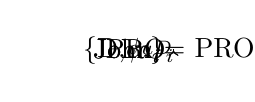
\begin{tikzpicture}[sibling distance=0pt]
\tikzset{level distance=25pt}
\Tree [.TP \node(a){John$_i$}; [.T' T [.vP \node(b){\sout {John$_i$}}; [.v' [.v managed v ] [.VP {t$_v$} [.FinP \node(d){PRO$_i$}; [.Fin' Fin[$_{uD}$] [.TP \node(c){\{D,$\phi$:\}= {\sout PRO$_i$}}; [.T' to [.vP \edge[roof]; {stay healthy} ] ] ] ] ] ] ] ] ] ]
\draw[->, to path={-| (\tikztotarget)}]
  (b) edge (a) ;
\draw[->, to path={-| (\tikztotarget)}]
  (c) edge (d);
\end{tikzpicture}
}
\caption{Subject complement control (Landau 2015: 26)}
\label{fig:sctree}
\end{figure}

\largerpage
Under Landau’s derivation of predicative control, object control occurs in complements with implicative verbs that are semantically causative (such as \textit{make}, \textit{compel}, \textit{force}). In object control constructions, the object, positioned in the subject position of a small clause (here an RP, which is a predicative or relator phrase), intervenes between the matrix subject and PRO and is the closest c-commanding DP to PRO. Only then can the object, rather than the subject, control PRO. The structure of object control, from \citet[29]{landau2015} is given below in \figref{fig:octree} for (\ref{octree}) with the controlling, intervening object in bold.

\ea \label{octree} John forced Bill to stay home. \jambox{\citep[29]{landau2015}}
\z

\begin{figure}
\scalebox{0.83}{
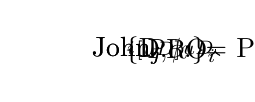
\begin{tikzpicture}[sibling distance=0pt]
\tikzset{level distance=25pt}
\Tree [.TP \node(a){John$_j$}; [.T' T [.vP \node(b){\sout {John$_j$}}; [.v' V [.VP force [.RP \textbf{Bill$_i$} [.R' Rel$_{[uD]}$ [.FinP \node(d){PRO$_i$}; [.Fin' Fin[$_{uD}$] [.TP \node(c){\{D,$\phi$:\}= {\sout {PRO$_i$}}}; [.T' to [.vP \edge[roof]; {stay home} ] ] ] ] ] ] ] ] ] ] ] ]
\draw[->, to path={-| (\tikztotarget)}]
  (b) edge (a) ;
\draw[->, to path={-| (\tikztotarget)}]
  (c) edge (d);
\end{tikzpicture}
}
\caption{Object complement control (Landau 2015: 29)}
\label{fig:octree}
\end{figure}


While \citet{landau2015} focuses mainly on deriving complement control structures, there is a brief discussion of extending his analysis to cases of adjunct control. Landau, following from \citet{williams1992}, claims that right-edge adjuncts function as predicates and display obligatory control, which in the TTC, are considered to be instances of predicative control. Regarding the technical details of predicative adjunct control, \citet{green2018adjunct} brings up questions regarding how the λ-operator is passed up the tree, since FinP is not the sister of any argument. He also questions how exactly predication is mediated in the adjunct. Like Green, I assume that these details can be worked out, and that the predication does obtain. I  refer the reader to \citet{landa2021} where a detailed analysis of adjunct control is provided. An example of the general structure for adjunct control following \citeauthor{landau2015} (\citeyear{landau2015}, \citeyear{landau2017}) is provided in \figref{fig:actree} for (\ref{actree}).

\ea \label{actree} John left after eating dinner.
\z

\begin{figure}
\scalebox{0.9}{

\begin{tikzpicture}[sibling distance=0pt]
\tikzset{level distance=25pt}
\Tree  [.TP \node(a){John$_i$}; [.T' T [.vP [.vP \edge[roof]; \node(b){\sout{ John$_i$} left};] [.PP after [.FinP \node(d){PRO$_i$}; [.Fin' Fin[$_{uD}$] [.TP \node(c){\{D,$\phi$:\}= {\sout {PRO$_i$}}}; [.T' T [.vP \edge[roof]; {eating dinner} ] ] ] ] ] ] ] ] ]
\draw[->, to path={-| (\tikztotarget)}]
  (c) edge (d);
  \draw[->, to path={-| (\tikztotarget)}]
  (b) edge (a);
\end{tikzpicture}
}
\caption{Adjunct control}
\label{fig:actree}
\end{figure}




\section{Control by object clitics} \label{Section 3}
In \sectref{section3.1} I first provide a brief overview of the distribution and analysis of object clitics in Spanish that I will adopt and lay out the structure I assume for them. Following, in \sectref{Section3.2} I discuss in more detail the contexts in which clitic control into adjuncts can obtain in Spanish, followed by a discussion of the type of control displayed in these structures in \sectref{section3.3}.
\subsection{Background on Spanish clitics} \label{section3.1}
In Spanish, accusative clitics can be located in different positions, depending on the structure of the sentence. With finite verbs, clitics are obligatorily located in a preverbal position (\ref{8b}). However, when the verb immediately preceding the clitic is an infinitive or gerund form of the verb, the clitic can optionally remain in-situ (\ref{8c}) or can be positioned before the inflected verb (\ref{8d}). The position in between the finite and non-finite verb is, however, not available for the
clitic (\ref{8e}). These positions are summarized below.

\ea \label{cliticpositions}
\ea \label{8a}
{
\gll Juan comió el pan. \\
Juan ate.\textsc{3sg} the bread \\
\glt ‘Juan ate the bread.’
}
\ex \label{8b}
{
\gll Juan lo$_i$ comió \textit{t$_i$}. \\
Juan it ate.\textsc{3sg} \\
\glt ‘Juan ate it.’
}
\ex \label{8c}
{
\gll Juan está comiendo-lo. \\
Juan is.\textsc{3sg} eating-it \\
\glt ‘Juan is eating it.'
}
\ex \label{8d}
{
\gll Juan lo$_i$ está comiendo \textit{t$_i$}. \\
Juan it is.\textsc{3sg} eating \\
\glt ‘Juan is eating it.’
}
\ex \label{8e}
{
\gll *Juan está lo$_i$ comiendo \textit{t$_i$}.\\
Juan is.\textsc{3sg} it eating \\
\glt ‘Juan is eating it.’
}
\z
\z

Regarding the structural position of these clitics, I assume the clitics are originally merged in the internal argument position before moving into their preverbal position. Following phase theory (\citealt{chomsky2000minimalist}, \citeyear{chomsky2001derivation}) and phase-based approaches to cliticization (\citealt{gallego2016phase}), I assume that the clitic is first moved through the edge of the vP phase, before moving to its final position. Making use of the notion of tucking-in following \citet{richards1997moves}, I consider the object clitics to be merged in the argument position and then tucked into an inner specifier following \citet{nevins2011multiple} and \citet{kramer2014clitic} (however, see \sectref{section4.3} for an update to this analysis). The basic structure of (\ref{8b}) is illustrated in (\ref{9}).

\ea \label{9}
{[{$_\textsc{TP}$} \textit{pro} [{$_\textsc{TP}$} lo comió [{$_\textsc{vP}$} \sout{lo} \textit{\sout{pro}} \textit{v} [{$_\textsc{VP}$} \sout{comió} \sout{lo}]]}
\z

\subsection{Clitic control data} \label{Section3.2}

In this section I present more examples of clitic control and outline the range of structures and clitic types that allow for this type of adjunct control construction. For this paper, I am limiting the scope of the discussion to only right-edge (i.e. final) temporal adjuncts which are traditionally claimed to only allow subject (not object) control.\footnote{Object and subject purpose adjuncts can display object control, where PRO is controlled by the goal or benefactive, as in (\ref{a}).
\ea \label{a} {We bought Mary$_i$ the dog [PRO$_i$ to play with].}
\z
\ea \label{b} {She called a detective$_i$ [PRO$_i$ to investigate the affair]. \jambox{(\citealt{landau2013})} }
\z
While discussed in detail in \citet{faraci1974aspects}, \citet{chomsky1980binding} and \citet{jones1991purpose}, a key difference between purpose and temporal adjuncts is that purpose adjuncts are argued to be attached in a lower position, as VP (internal) adjuncts (see also \citealt{green2019movement} for a discussion of adjunct height). This position would make \textit{Mary} in (\ref{a}) and \textit{a detective} in (\ref{b}) the closest c-commanding controller. This lower position can account for why an object, and not the subject, is the obligatory controller.} The example from (\ref{clitcctl}) is repeated below in (\ref{clitic3person}), along with additional examples of clitics controlling the adjunct subject.

\ea \label{clitcctl2}
\ea \label{clitic3person}
{
\gll \textbf{La$_{i}$} besé después de PRO$_{i}$ ponerse celosa.\\
her kissed after of PRO became.\textsc{inf.refl.3sg} jealous.\textsc{f}\\
\glt `I kissed her after she got jealous.'
}
\ex \label{clitic2person}
{
\gll ¿Tu novio no \textbf{te$_i$} vio antes de PRO$_i$ irte para la boda? \\
your boyfriend didn’t you see.\textsc{3sg} before of PRO leave.\textsc{inf.refl.2sg} for the wedding \\
\glt ‘Your boyfriend didn’t see you before you left for the wedding?’
}
\ex \label{clitic1person}
{
\gll Mi papá \textbf{me$_i$} llevó para PRO$_i$ comenzar el primer día de escuela.\\
my dad me brought to PRO start.\textsc{inf} the first day of school\\
\glt ‘My dad brought me to start my first day of school.’
}
\z
\z

As seen from these examples, third person clitics (\ref{clitic3person}), as well as second (\ref{clitic2person}), and first person clitics (\ref{clitic1person}) are all able to control into an adjunct. Note that while the controlled verb in both (\ref{clitic3person}) and (\ref{clitic2person}) is reflexive in order to show an overt realization of the features of the controller, this is not obligatory, as displayed in (\ref{clitic1person}) and later in (\ref{inanimate}), where the controlled verb is not reflexive. In these structures, PRO is the antecedent of the reflexive, and the reflexive pronoun thus indicates which argument is controlling PRO. While the data in (\ref{clitcctl2}) show that clitic control is possible, crucially, as was shown in (\ref{cliticsubjctl}), subject control is still possible into these Spanish temporal adjuncts. Observe the minimal pair in (\ref{minimalpair}) where both subject and clitic control are possible.


\ea \label{minimalpair}
\ea \label{minimalpairS}
{
\gll (\textbf{Yo$_j$}) lo vi antes de PRO$_j$ irme para España. \\
I him saw.\textsc{1sg} before of PRO leave.\textsc{inf.refl.1sg} for Spain\\
\glt ‘I saw him before (my) leaving for Spain.’
}
\ex \label{minimalpairC}
{
\gll (Yo) \textbf{lo$_i$} vi antes de PRO$_i$ irse para España. \\
I him saw.\textsc{1sg} before of PRO leave.\textsc{inf.refl.3sg} for Spain\\
\glt ‘I saw him before he left for Spain.’
}
\z
\z

Thus, it appears that these clitic control structures involve some degree of optionality as to which argument, the subject or the object clitic, acts as the controller. I return to this optionality in \sectref{Section 4}.


Further, while the object clitic controls PRO in the structures in (\ref{clitcctl2}), it is important to note that this only appears to be possible when the object is a clitic, rather than a full DP, and crucially, only when the clitic is moved to a preverbal position. Observe how postverbal DPs (both full DP objects and object clitics) cannot control, shown in (\ref{insituobj}) and (\ref{postverbalcl}). Additionally, postverbal clitics in imperative structures are also unable to establish control (\ref{imperative}) as are preverbal clitics in clitic climbing structures (non clause-mate clitics) (\ref{cliticclimbing}).

\ea \label{ungrammatical}
\ea[*]{
\gll Besé [a mi novia]$_i$ antes de PRO$_i$ ponerse celosa.\\
kissed \textsc{dom} my girlfriend before of PRO become.\textsc{inf.refl.3sg} jealous.\textsc{f}\\
\glt ‘I kissed my girlfriend before she got jealous’
}\label{insituobj}
\ex[*]{
\gll Quiero besar-la$_i$ antes de PRO$_i$ ponerse celosa.\\
want.\textsc{1sg} kiss.\textsc{inf}-her before of PRO become.\textsc{inf.refl.3sg} jealous.\textsc{f}\\
\glt ‘I want to kiss her before she gets jealous.’
}\label{postverbalcl}
\ex[*]{
\gll Bésa-la$_i$ antes de PRO$_i$ irse.\\
kiss-her before of PRO leave.\textsc{inf.refl.3sg}\\
\glt ‘Kiss her before she leaves.'
}\label{imperative}
\ex[*]{
\gll Lo$_i$ logré conocer antes de PRO$_i$ graduarse.\\
Him managed meet.\textsc{inf} before of PRO graduate.\textsc{inf.refl.3sg}\\
\glt ‘I managed to meet him before he graduated.’
}\label{cliticclimbing}
\z
\z

 The full DP object, \textit{mi novia}, in (\ref{insituobj}) is unable to control the adjunct subject. Likewise, the example in (\ref{postverbalcl}) shows that an accusative in-situ clitic also cannot be interpreted as the adjunct subject.  The full DP object and postverbal clitic and examples appear parallel to the English example in (\ref{obctladj}), in that a lower internal argument is unable to control. I return to discuss these ungrammatical examples, including the imperative structure in (\ref{imperative}) and (\ref{cliticclimbing}), where the clitic in a higher clause is unable to control, in \sectref{section4.3}. Note that in order for (\ref{insituobj}) and (\ref{postverbalcl}) to have the desired interpretation, both examples would require the use of the subjunctive in the adjunct verb, in which case the subject would be considered \textit{pro}, since the verb would no longer be a non-finite form, shown in (\ref{subjunctive}).

\ea \label{subjunctive}
\gll Besé a mi novia$_i$ después de que \textit{pro$_i$} se pusiera celosa.\\
kissed \textsc{dom} my girlfriend after of that \textit{pro} \textsc{se} became.\textsc{subj} jealous.\textsc{f}\\
\glt ‘I kissed my girlfriend after she got jealous.’
\z

The conclusion from this data is summarized in (\ref{summaryofcliticctl}).\footnote{It is important to mention another structure where a non-(nominative) subject, dative experiencers, can control into temporal adjuncts, as in (\ref{dative}).
\ea \label{dative}
{
\gll Siempre me$_i$ duele la cabeza$_j$ después de PRO$_{i/*j}$ correr.\\
always \textsc{1sg.dat} hurts the head after of PRO run.\textsc{inf}\\
\glt `My head always hurts after running.'
}
\z
Because of the structural differences between these experiencer constructions and the examples in (\ref{clitcctl2}), I set aside these constructions. For a full discussion of control by dative experiencers see \citet{landau2009} as well as \citet{landa2021}. These may fall under the category of NOC.}

\ea \label{summaryofcliticctl}
Only moved, clause-mate, pre-verbal clitics are potential object controllers of the subject position of non-finite adjuncts in Spanish.
\z

\subsection{Clitic control is OC not NOC} \label{section3.3}
As a final discussion before proceeding into the analysis of clitic control, it is important to
establish what type of adjunct control these clitic structures display, obligatory control (OC) or non-obligatory control (NOC). While OC structures are controlled by a local antecedent, NOC structures are those where PRO is not syntactically bound by a local antecedent in the structure, but rather PRO refers to a long-distance antecedent, a discourse referent, or an arbitrary referent \citep{landau2013}. Thus, NOC is subject to fewer syntactic constraints on the controller. Three typical examples of NOC, arbitrary control, long distance control, and discourse control (all from \citealt{landau2013}), are given in (\ref{NOC}).

\ea \label{NOC}
\ea \label{NOCarb}
{
Potatoes are tastier [after PRO$_{Arb}$ boiling them.]\\  
\jambox{(Arbitrary NOC)}
}
\ex \label{NOCld}
{
We$_i$ thought that [PRO$_{j/i}$ to expose herself/ourselves] would help Mary$_j$. \jambox{(Long distance NOC)}
}
\ex \label{NOCdisc}
{
Clearly, [PRO confessing my crime] was not something they anticipated. \jambox{(Discourse NOC)}
}
\z
\z

In (\ref{NOCarb}) the subject of the matrix clause, potatoes, is not interpreted as controlling PRO, but instead PRO, not being controlled by any syntactic antecedent, receives an arbitrary interpretation. In (\ref{NOCld}) PRO refers to a long-distance antecedent by which it is not bound. Likewise, (\ref{NOCdisc}) is also not bound by an element in the structure but instead receives its interpretation from something salient in the discourse.


In this section, I address if it is possible to analyze constructions like (\ref{clitcctl2}) as instances of NOC, rather than OC. Classifying these structures as NOC would be a way to avoid the questions that arise regarding accounting for clitic control mentioned in \sectref{Section1}. However, I show that this approach is not tenable. The clitic control structures do display the characteristics of OC.


\citet{landau2017} expands on his discussion of adjunct control from \citet{landau2015} and suggests that right-edge (final) adjuncts can be either OC or NOC. The central claim is that while OC right-edge adjuncts are derived via predication, NOC right-edge adjuncts are derived via logophoricity. The difference, Landau claims, between OC and NOC final adjuncts relies heavily on the presence (or absence) of a c-commanding controller. While OC PRO must be bound by a local antecedent and must be interpreted as a bound variable, NOC PRO may be a free variable and does not need to be bound by another element. It is also standardly claimed that NOC PRO is obligatorily [+human]. The summary of what Landau refers to as the OC/NOC signature is given in (\ref{OCsig}) and (\ref{NOCsig}).

\ea \label{OCsig}
The OC signature\\
In a control construction [...Xi ...[s PRO$_i$ ...]...], where X controls the PRO subject of the clause S:
\ea \label{OCa} {The controller(s) of X must be (a) codependent(s) of S.\footnote{\citet{landau2013} defines a codependent as: “A ‘dependent’ of S is either an argument or an adjunct of S, thus (a) subsumes both complement OC, where the controller and S are co-arguments and adjunct OC.”}}
\ex \label{OCb} {PRO (or part of it) must be interpreted as a bound variable.}
\z
\z


\ea \label{NOCsig}

The NOC signature\\
In a control construction [...[s PRO$_i$ ...]...]:
\ea \label{NOCa} {The controller need not be a grammatical element or a co-dependent of S.}
\ex \label{NOCb} {PRO need not be interpreted as a bound variable (i.e., it may be a free variable)}
\ex \label{NOCc} {PRO is [+human].\hfill (\citealt{landau2013})}
\z
\z
Thus, if one were to classify structures like (\ref{clitcctl2}) as displaying NOC, clitic control would not
immediately be problematic for predication-based (or the earlier AGREE-based) theories of control. There are, however, examples of object clitic control structures that clearly do not fit into Landau’s definition of the NOC signature.


Examining the first criteria, (\ref{OCa}), the clitic controller in examples like (\ref{clitcctl2}) is a co-dependent of S, satisfying that requirement of the OC signature. However, while in NOC the controller is not obligatorily a co-dependent but may be a co-dependent of S, being a co-dependent of S does not rule out (\ref{clitcctl2}) being NOC. Turning to the [+human] aspect of the NOC signature, observe (\ref{inanimate}) where a non-human object can control PRO.


\ea \label{inanimate}
\ea
{
\gll La$_i$ tiré después de PRO$_i$ estar en la mesa por dos semanas. (la=la carta) \\
it threw-away after of PRO be.\textsc{inf} on the table for two weeks. (it=the letter) \\
\glt ‘I threw it away after it was on the table for two weeks.’ (where ``it" refers to ``the letter")}
\ex{
\gll Lo$_i$ cosechó antes de PRO$_i$ florecer. \\
it harvested before of PRO flower.\textsc{inf} \\
\glt ‘He/She harvested it before it flowered.’}
\z
\z

\largerpage[-1]
According to Landau’s NOC signature, NOC PRO should only be interpreted as human. However, in (\ref{inanimate}) an accusative, non-human clitic can control PRO, showing that these structures do not conform to the requirements of NOC. Moreover, if the structures in (\ref{clitcctl2}) were instances of NOC, rendering a c-command relationship unnecessary, it would not be immediately clear why postverbal clitics or non-clause mate preverbal clitics cannot control. If the dependency were not local, and c-command were not a requirement, why would only preverbal clitics control? Therefore, following Landau’s definition of the OC/NOC signature, there is strong support for treating these structures as OC.


In sum, from the data and discussion in this section, I conclude that in addition to matrix subjects being able to control adjunct PRO, preverbal clitics (either 1st, 2nd, or 3rd person) are also able to control into an adjunct. Moreover, I have also shown that these structures are instances of obligatory control, rather than non-obligatory control. This is crucial to the discussions in the upcoming sections, where I account for the clitic control data under the assumption that these are cases of obligatory control.

\section{Clitic control in the TTC} \label{Section 4}
\largerpage[-1]
Because clitic control data like (\ref{clitcctl2}) are not discussed in previous theories of control, and in fact obligatory control by an object is not predicted to occur at all in temporal adjuncts, further explanation is needed to account for these structures. In \sectref{section4.1}, I discuss how clitic control examples can be analyzed under \citeauthor{landau2015}'s (\citeyear{landau2015}) theory of control. In \sectref{section4.2} I propose a way to account for the optionality between subject and object clitic control into adjuncts based on the position of the subject and clitic. Finally, in \sectref{section4.3}, I return to the ungrammatical clitic control examples mentioned in \sectref{Section3.2} and show how those can also be accounted for under the TTC.

\subsection{Accounting for clitic control} \label{section4.1}
Following the framework of the TTC presented in \citet{landau2015}, the lack of object control in temporal adjuncts would likely be attributed to the fact that an internal argument in the matrix would not be able to c-command the adjunct, and thus no predication could be attained between PRO and the controller. While this would correctly rule out the ungrammatical examples involving full DP objects (in both English and Spanish) there still appears to be room in this theory to also account for the examples where an object clitic can successfully control into an adjunct.\footnote{\citet{janke2017} claim that not all temporal adjuncts are obligatorily controlled by the subject but that pragmatics can influence the choice of controller to instead be the matrix object. In an experimental study, they found that in a control structure with a final temporal adjunct, when strongly primed in the preceding discourse, almost half of speakers understood the matrix object to be the controller in an example like (\ref{HPcontrol}).
\ea \label{HPcontrol} Hermione is looking after the birds. Hermione takes out the food. Ron tapped Hermione while feeding the owl.
\z
Because the both controller options are [+human] it is not immediately clear that this is an OC interpretation. However, if these can be analyzed as displaying OC with an object controlling, this may then serve as a counterexample to the traditional generalization that objects cannot control into adjuncts.} In Landau’s theory, it is the final position of the object that is argued to block object control in English adjuncts. When no c-command relationship can be established between the controller and controlee under this theory, predication, and consequently Control, fail to occur. However, recall from the discussion in \sectref{Section 3} that Spanish (preverbal) clitics are moved to a higher position. From this higher position in Spec vP, the clitic is able to c-command and saturate the predicate of the adjunct subject, which is what appears to allow the object control to occur. In this case, predication (and thus control) can be established between the controller (the clitic) and PRO. Moreover, on the account that the clitic tucks into an inner specifier of vP, there appears to be no other argument intervening between the clitic and PRO. Observe the structure of (\ref{clitic3person}) shown below in \figref{fig:cctree} for (\ref{cctree}).\footnote{Thanks to Idan Landau for his input on this structure.}

\ea \label{cctree} {La besé después de ponerse celosa.}
\z

\begin{figure}
\scalebox{0.8}{
\begin{tikzpicture}[sibling distance=0pt]
\tikzset{every tree node/.style={align=center,anchor=north}}
\tikzset{level distance=25pt}
\Tree [.TP DP\\{\textit{pro}} [.TP DP\\la [.T' T\\besé [.vP DP\\{\sout{\textit{pro}}} [.vP DP\\{\sout{la}} [.vP [.v' v\\{\sout{besé}} [.VP V\\{\sout{besé}} [.DP\\{\sout{la}} ] ] ] [.PP {P\\{después de}} [.FinP PRO [.Fin' Fin [.TP \edge[roof]; {\sout{PRO} ponerse celosa} ] ] ] ] ] ] ] ] ] ]
\end{tikzpicture}
}
\caption{Clitic control}
\label{fig:cctree}
\end{figure}

The structure in \figref{fig:cctree} can thus account for the phenomenon of clitics controlling. However, we are then left with a larger question regarding how both subject and clitic control are possible in an otherwise identical structure (as in (\ref{minimalpair})). While the structure and analysis in \figref{fig:cctree} demonstrates how preverbal Spanish clitics are able to establish predication with PRO, this analysis consequently predicts that only the clitic could act as a controller of PRO, given that it intervenes between the matrix subject and PRO. This then raises questions regarding the structure of subject control into adjuncts and how it is possible for either the subject or object to be the controller. I now turn to discussing how to account for this possibility of both subject and clitic control.


\subsection{Co-existence of subject and clitic control into adjuncts} \label{section4.2}

Recall that subject control is also possible in the structures with preverbal clitics, as was
shown in the minimal pair in (\ref{minimalpair}), and repeated below in (\ref{minimalpair2}).

\ea \label{minimalpair2}
\ea \label{minimalpairS2}
{
\gll (\textbf{Yo$_j$}) lo vi antes de PRO$_j$ irme para España. \\
I him saw.\textsc{1sg} before of PRO leave.\textsc{inf.refl.1sg} for Spain\\
\glt ‘I saw him before (my) leaving for Spain.’
}
\ex \label{minimalpairC2}
{
\gll (Yo) \textbf{lo$_i$} vi antes de PRO$_i$ irse para España. \\
I him saw.\textsc{1sg} before of PRO leave.\textsc{inf.refl.3sg} for Spain\\
\glt ‘I saw him before he left for Spain.’
}
\z
\z

\largerpage[-2]
\noindent The possibility of both subject and clitic control suggests that there is some amount of optionality in the controller of an obligatory control structure. This raises the questions of how this optionality arises and what determines which argument (the subject or the object clitic) is the controller. The idea of optionality in an obligatory control construction at first may seem unexpected given that in other examples of obligatory complement and adjunct control, there appears to never be optionality between subject and object control in the same structure.\footnote{There are some adjunct control structures that show optionality in that they can display either OC or NOC (discussed in detail in \citealt{green2018adjunct}, \citeyear{green2019movement}). Observe (\ref{greenexamp}), from \citet{green2018adjunct}, where the referent of PRO could be the subject (OC), or an antecedent outside of the sentence (NOC).
\ea \label{greenexamp}
{
The pool$_i$ was the perfect temperature after PRO$_{i/j}$ being in the hot sun all day.
}
\z
However, given the discussion in \sectref{section3.3}, where I have claimed that the clitic control examples do behave as OC, these structures are different than those like (\ref{greenexamp}) that show alternation between OC/NOC, as this alternation appears to be one between OC subject control and OC object control.} Observe (\ref{engexamp2}), from \citet{landau2015}, where in the presence of a matrix object in a predicative control structure, the object must control.

\ea \label{engexamp2}
\ea \label{21a}
John$_i$ managed PRO$_i$ to stay healthy. \jambox{(Subject control)}
\ex \label{21b}
John$_i$ forced Bill$_j$ PRO$_{*i/j}$ to stay home. \jambox{(Object control)}
\z
\z


However, the adjunct control structures are quite different than those of complement control in (\ref{engexamp2}). With a subject control verb like \textit{manage} in (\ref{21a}), the only available interpretation is with the subject \textit{John} acting as the controller. \textit{John}, the subject, is the only c-commanding DP. There is no competing or intervening DP, and thus the subject controls PRO. On the other hand, in (\ref{21b}), the matrix object must be the controller of PRO. For predicative control, all object control structures (primarily those non-attitude verbs that are semantically causative) are always controlled by the object. As discussed in \sectref{Section 2}, in these cases the predicative head (FinP) applies to the small clause that contains the matrix object. The object in these cases is the closest, c-commanding DP which saturates the predicate (PRO) and will always control. Thus, because of the structure of complement control constructions, no optionality can arise between subject and object control.


I propose that the optionality in subject/clitic control arises from the position of the clitic. Until now, I have assumed for this analysis that the clitic moves to Spec vP, tucked in under the external argument, which is also in a specifier of vP. However, the two different semantic interpretations (subject control vs object clitic control), leads to the natural suggestion of there being two distinct derivations for these structures. In both derivations, the subject would move first, to the specifier of vP. Following, in the derivation resulting in clitic control, the clitic would tuck-in to an inner specifier of vP, as was claimed earlier. In this derivation, the clitic would be the closest c-commanding DP to PRO and would thus saturate the predicate in the adjunct and establish control. However, I argue that an alternate derivation is also possible which results in subject control. In this derivation, instead of the clitic tucking-in, it would move to an outer specifier of vP. Here the subject would instead be the closer DP to PRO and would thus serve as the controller. Following \cite{richards1997moves}, both of these derivations (movement to an outer specifier or tucking into an inner specifier) in principle should be possible, and both respect notions of cyclicity as outlined in \citet{chomsky19954minimalist}. This possibility of optionality in the derivation (i.e. clitic movement to outer specifier or tucking into an inner specifier) also conforms to the notion in \citet[34]{chomsky2001derivation} that optionality is allowed if it leads to a different outcome, i.e. a difference in the interpretation (in this case subject vs object control).\footnote{An alternative explanation for the alternation between subject and clitic control was suggested by an anonymous reviewer, wherein if the clitic and subject are both in multiple specifiers, they would remain equidistant from PRO and neither would block the other. While this would be a simpler solution, this type of optionality, however, would not be expected under an analysis for control that is derived via predication, like the TTC. With predication, it is expected that only one, closest controller will saturate the predicate and establish control.} Simplified versions of these two derivations are shown in \figref{ccCtree} and \figref{ccStree}, using the examples from (\ref{minimalpair2}).\footnote{For reasons of clarity, and in order to focus on the clitic movement, I have simplified the structures in \figref{treederiv}. Here, I adopt an account of Spanish subjects in which overt, preverbal subjects are found in a higher position than pro, along the lines of \citet{cardinalettiRoberts} and \citet{cardinaletti1997}. Specifically, I follow the account for Spanish subjects from \citet{suner2003lexical}, who makes use of multiple specifier positions and proposes that Spanish overt subjects are in an upper specifier of TP, higher than null subjects. This structure would be as is shown in (\ref{suner}).
\ea \label{suner} [TP yo [TP pro [ V...]]]
\z
Thus, in these cases, if the subject is pronounced, it would be moved to a higher specifier of TP, but the lower deleted copy/trace in the Spec vP position is what saturates the predicate and establishes control. With this analysis of subjects taken into account, the derivation results in the desired word order.}


\begin{figure}
\begin{subfigure}{\textwidth}

\begin{tikzpicture}[sibling distance=0pt]
\tikzset{every tree node/.style={align=center,anchor=north}}
\tikzset{level distance=25pt}
\Tree [.TP DP\\yo [.TP DP\\lo [.T' T\\vi [.vP DP\\{\sout{yo}} [.vP DP\\{\sout{\textbf{lo}}} [.vP [.v' v\\{\sout{vi}} [.VP V\\{\sout{vi}} [.DP\\{\sout{lo}} ] ] ] [.PP \edge[roof]; {antes de PRO irse} ] ] ] ] ] ] ]
\end{tikzpicture}
\caption{Clitic control: tucking-in derivation}
\label{ccCtree}
\end{subfigure}
\begin{subfigure}{\textwidth}

\begin{tikzpicture}[sibling distance=0pt]
\tikzset{every tree node/.style={align=center,anchor=north}}
\tikzset{level distance=25pt}
\Tree [.TP DP\\yo [.TP DP\\lo [.T' T\\vi [.vP DP\\{\sout{lo}} [.vP DP\\{\sout{\textbf{yo}}} [.vP [.v' v\\{\sout{vi}} [.VP V\\{\sout{vi}} [.DP\\{\sout{lo}} ] ] ] [.PP \edge[roof]; {antes de PRO irme} ] ] ] ] ] ] ]
\end{tikzpicture}
\caption{Subject control: clitic movement to outer specifier derivation}
\label{ccStree}
\end{subfigure}
\caption{Clitic vs subject control derivations}
\label{treederiv}
\end{figure}

If the existence of both subject and clitic control is made available from the possibility of two different derivations as I have suggested above, instances of optionality between a clitic and subject would be expected to be found in other structures, outside of the adjunct control examples. One such situation is observed with reflexive binding, where both the clitic and subject are able to serve as the antecedent to the reflexive pronoun, shown in (\ref{binding}).
\ea \label{binding}
\ea[]{
\gll Le hablé de mí-mismo. \\
him spoke.\textsc{1sg} of myself \\
\glt ‘I talked to him about myself.’}\label{bindinga}
\ex[]{
\gll Le hablé de sí-mismo. \\
him spoke.\textsc{1sg} of himself \\
\glt ‘I talked to him about himself.’}\label{bindingb}
\ex[*]{
\gll *Hablé a Juan de sí-mismo. \\
spoke.\textsc{1sg} to Juan of himself \\
\glt ‘I talked to Juan about himself.’}\label{bindingc}
\z
\z

In the examples in (\ref{binding}), a local c-commanding antecedent is needed to bind reflexives. In (\ref{bindinga}), the first-person reflexive anaphor \textit{mí mismo} is bound by the first-person (null) subject. In (\ref{bindingb}), the third-person reflexive \textit{sí mismo} is bound by the third-person clitic, \textit{le}. Finally, in (\ref{bindingc}), the third person reflexive anaphor is not licensed due to the lack of an appropriate binder that has matching features. The full DP \textit{Juan} does not c-command the anaphor, leading to the ungrammaticality. I thus conclude from (\ref{binding}) that there is a choice between the two potential binders, either the clitic or the subject. This suggests that, similar to the adjunct control cases, with reflexive binding, there are two derivations possible. Either the clitic tucks in, and is the closest DP for control/binding, or the clitic moves to an outer specifier, and the subject then is the closest DP. Therefore, the optionality between the two derivations does not appear to be limited to just the adjunct control structures.


Finally, the proposal that the clitic and the subject are both possible controllers, depending on the derivation, should not cause a problem under the framework set up in the TTC. There seems to be no theoretical motivation to exclude the possibility of two DPs being potential controllers.\footnote{A potential parallel would be in cases with split control, where the reference of PRO includes both the subject and the object, as well as partial control, where the reference of PRO is only partially included in the controller. Observe an example of partial control in Spanish, below.
\ea
\gll La abracé después de PRO reunirnos por primera vez. \\
her hugged after of PRO meet.\textsc{inf.1pl} for first time \\
\glt ‘I hugged her after we met for the first time.’
\z
However, both split and partial control, following \citet{landau2015}, involve logophoric control rather than predicative control (since, per Landau, predication cannot be partial). These do appear different than the earlier examples of clitic control, crucially because a parallel structure, but with an in-situ direct object, is also grammatical.
\ea
\gll Abracé a mi hermana después de PRO reunirnos por primera vez. \\
hugged \textsc{dom} my sister after of PRO meet.\textsc{inf.1pl} for first time \\
\glt ‘I hugged my sister after we met for the first time.’
\z
Due to the differences in the structure of predicative and logophoric control though, crucially that logophoric control involves variable binding which gives the reference of PRO to either the addressee or author (or in the case of partial control, both), this is not a direct parallel.} I thus conclude that while it may not be seen in other cases of obligatory control, with the appropriate structure, there is the possibility of controller optionality in adjunct control. This still conforms to the TTC as there is nothing that explicitly rules out the possibility for optionality.


\subsection{Explaining the ungrammatical clitic control examples} \label{section4.3}

Lastly, in addition to explaining the grammatical clitic control examples in (\ref{clitcctl2}), the TTC can also successfully account for the ungrammatical object control examples, as shown in (\ref{ungrammatical}), and repeated below in (\ref{ungrammatical2}).

\ea \label{ungrammatical2}
\ea[*]{
\gll Besé [a mi novia]$_i$ antes de PRO$_i$ ponerse celosa.\\
kissed \textsc{dom} my girlfriend before of PRO become.\textsc{inf.refl.3sg} jealous.\textsc{f}\\
\glt ‘I kissed my girlfriend before she got jealous.’
}\label{insituobj2}
\ex[*]{
\gll Quiero besar-la$_i$ antes de PRO$_i$ ponerse celosa.\\
Want.\textsc{1sg} kiss.\textsc{inf}-her before of PRO become.\textsc{inf.refl.3sg} jealous.\textsc{f}\\
\glt ‘I want to kiss her before she gets jealous.’
}\label{postverbalcl2}
\ex[]{
\gll Bésa-la$_i$ antes de PRO$_i$ irse.\\
kiss-her before of PRO leave.\textsc{inf.refl.3sg}\\
\glt ‘Kiss her before she leaves.'
}\label{imperative2}
\ex[*]{
\gll Lo$_i$ logré conocer antes de PRO$_i$ graduarse.\\
Him managed meet.\textsc{inf} before of PRO graduate.\textsc{inf.refl.3sg}\\
\glt ‘I managed to meet him before he graduated.’
}\label{cliticclimbing2}
\z
\z

The examples in (\ref{insituobj2}) and (\ref{postverbalcl2}) are accounted for straightforwardly in the TTC. As is suggested for the ungrammatical object control examples in English in (\ref{engexamp}), in (\ref{insituobj2}) and (\ref{postverbalcl2}) the in-situ object or clitic are likewise not in a position to c-command PRO in the adjunct. Thus, under this theory, given that predication is the crucial step in establishing control and an in-situ object cannot c-command the adjunct, these arguments are unable to establish predication and thus are unable to control.\footnote{There are various accounts proposing that objects with differential object marking (DOM) in Spanish are moved to a higher position, such as Spec {$\alpha$}P (between vP and VP) in \citet{lopez2014derivational}, Spec vP in \citet{torrego1998dependencies}, or even higher to Spec DatP in \citet{rodriguez2007syntax}. While it is outside of the scope of this paper to develop a specific account of DOM objects, due to the lack of full-DP objects, including DOM objects, controlling into adjuncts, I assume an account of DOM objects in which the adjunct is adjoined higher than whatever the final position of the DOM object ultimately is.} Once again, the positioning of the object clitic in Spec vP is crucial in allowing control to occur into an adjunct. I acknowledge that there may be further questions regarding the topic of clitic positions, particularly for the postverbal clitics (\ref{postverbalcl2}), as an anonymous reviewer points out. Given the considerable literature on Spanish clitics, and the lack of one established or standard account, in this paper I am assuming that the final position of postverbal clitics is low, and not in a position where it is in competition to be controller. However, note that even if a postverbal clitic is analyzed as having a final position in TP, this will be too high a position to control from, given that the subject (in Spec vP) is always expected to intervene. The topic is one that deserves more attention, and I set a more complex discussion of the issue aside as a question for future research.


Regarding (\ref{imperative2}), approaches like \citet{rivero1995imperatives} claim the obligatory postverbal position of the clitic in imperative structures arises from verb movement to C, which occurs around the raised clitic. If this account is correct, the ungrammaticality of (\ref{imperative2}) is unexpected, since the clitic is also found in TP in these structures. I follow \citet{terzi1999clitic} who says that in imperative structures, the clitic adjoins to T and the verb left incorporates into the clitic. It is then the verb and clitic complex that moves up to C, accounting for the clitic’s postverbal position. In this case, the clitic would then be higher in T/C, and the subject would be the closest controller, resulting in control only by the subject.


Finally, turning to (\ref{cliticclimbing2}), where there is a complement control structure in the matrix clause and the clitic climbs to be positioned before the inflected verb, the clitic is also unable to control into an adjunct. While I assume this arises due to the complications with the additional complement subject control clause in the matrix (\textit{Lo logré PRO conocer antes de PRO graduarse)}, I set aside a full account of this structure for future research.


Observe that from this data it can be concluded that while the object must be in a higher position (i.e. a preverbal clitic, rather than an in-situ full DP object or an in-situ object clitic), it also cannot be too high (as seen in the imperative example). That is, a specifier of vP is the crucial position. This can also be seen in examples with objects moved to the left periphery, where they are too high to control. For example, in interrogative structures like (\ref{question}), the object is moved to Spec CP, a position from which it could c-command PRO in the adjunct. However, only the subject is a possible controller.

\ea \label{question}
\gll ¿A quién$_i$ viste t$_i$ antes de PRO ir[te/*se] para España? \\
\textsc{dom} who see.\textsc{2sg} t before of PRO leave.\textsc{inf.[refl.2sg/refl.3sg]} for Spain? \\
\glt ‘Who did you see before (your) leaving for Spain?’
\z
When the object is moved to Spec CP, there is no derivation in which the object is in a position to control. The subject must be the closest c-commanding DP and is the only possible controller, as it would always intervene between the higher object and adjunct PRO. This reinforces the obligatory nature of the clitic being positioned in Spec vP as a precondition of being a potential controller of adjunct PRO.

\section{Conclusion} \label{Conclusion}
The goal of this paper was to contribute the novel observation that object clitics can control into Spanish adjuncts to the empirical discussion of adjunct control. Unlike what has been generally claimed, that only subjects can control into temporal adjuncts, preverbal, clause-mate object clitics in Spanish are potential controllers. Interestingly, the structures that allow clitic control alternatively allow for subject control as well. Thus, the dichotomy of when subject and object control occur appears to not be as strict as in complement clauses. I have argued that this optionality in the choice of controller is due to the position of the clitic, which has the option of either tucking into Spec vP or moving to an outer specifier of vP. When the clitic tucks in, it is the closest c-commanding DP to adjunct PRO and establishes control, but when it is moved to an outer specifier, the subject is closest to the adjunct and is the argument that establishes control.


\section*{Acknowledgements}
Thanks to two anonymous reviewers as well as audiences from LSRL 50 and Going Romance 34 for helpful feedback. Special thanks to Jonathan MacDonald, Aida Talić, Jefferey Green, Idan Landau, Yvette Bandín, Almike Vázquez-Lozares, Dulcinea Muñoz Gómez, Fabiola Fernandez Doig for data and discussion. All errors are my own.


\printbibliography[heading=subbibliography,notkeyword=this]

\end{document}
